\section{Systemüberblick}
Der in dieser Belegarbeit entstandene Entwurf basiert auf den 
Ideen von John D. Davis et al. \cite{davis:2008}. Es handelt sich um einen
applikationspezifischen Hybrid-Solver. Jedoch weicht er an einigen 
Stellen von dem ursprünglichen Design ab. So können wesentlich weniger
Variablen bearbeitet werden, es werden keine neuen Klauseln gelernt,
die Inferenz arbeitet mit Arbitern und der zugrunde liegende Suchalgorithmus ist DPLL statt CDCL. \\
Die Anzahl von Variablen, welche bearbeitet werden können,
ist geringer, da nur die auf dem FPGA befindlichen Block-RAMs genutzt werden.
Im ursprünglichen Entwurf wird zusätzlich noch ein DRAM-Speicher genutzt.
Auf die Nutzung von CDCL wurde verzichtet, weil der Algorithmus keinen Einfluss
auf den Inferenzprozess hat, sondern den Suchbaum anders als der DPLL-Algorithmus erzeugt.\\
In diesem Abschnitt werden die einzelnen Komponenten bzw. Module
des Entwurfs erläutert. In der folgenden Abbildung \ref{system} ist der Entwurf 
vereinfacht skizziert, um einen Überblick über das Gesamtsystem zu geben.
\begin{figure}[h]
  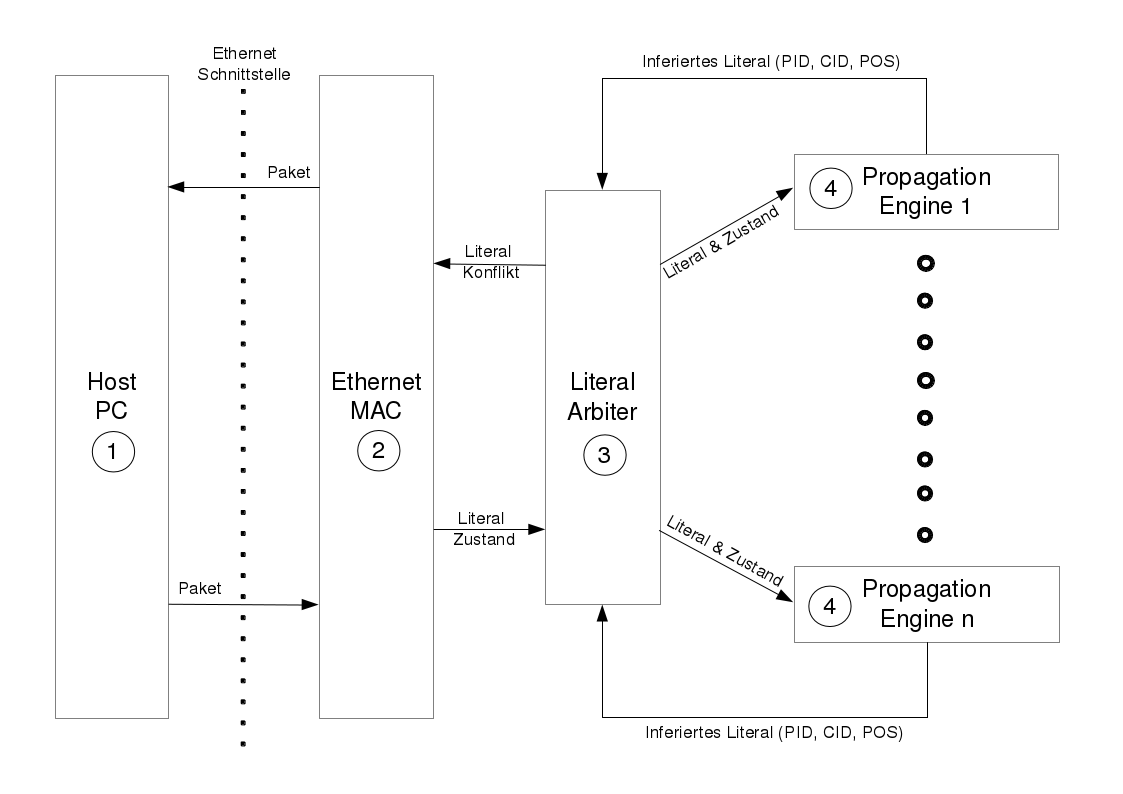
\includegraphics[width=\textwidth]{abb/system.png}
  \caption{Systemüberblick}
  \label{system}
\end{figure}
Ziel des Systems ist es, Entscheidungsliterale des Host-PCs so lange zu propagieren,
bis keine weiteren Literale propagiert werden können oder es zu einem 
Konflikt kommt. Im Konfliktfall muss vom Host-PC ein Rücksprung auf der
partiellen Interpretation durchgeführt und dem FPGA mitgeteilt werden.
Andernfalls muss der FPGA mit neuen Entscheidungsliteralen versorgt werden.\\
Es können mit diesem Entwurf Formeln mit bis zu 256 Variablen und 
4096 Klauseln gelöst werden. Eine Klausel darf dabei nicht mehr
als 9 Literale beinhalten. 
Die Variablen- und Klauselanzahl wird dabei durch die verfügbaren 
Block-RAM-Speicherressourcen der Literal-Übersetzungstabelle 
im Literal-Arbiter begrenzt.

\begin{enumerate}
\item Host-PC \newline
  Der Host-PC gruppiert die zu lösende Formel, übernimmt die Berechnung 
  von Entscheidungsliteralen und bestimmt den Rücksprungpunkt bei Konflikten.
  Er ist über eine Ethernet Schnittstelle 
  mit dem FPGA verbunden und kommuniziert mit diesem über Ethernet-Pakete.
  Mithilfe dieser Pakete steuert der Host-PC die Funktion des FPGAs.
\item Ethernet-MAC (Media Acces Control) \cite{xilinxether:2011}\newline
  Der Ethernet-MAC nimmt die Pakete des Host-PCs entgegen, verarbeitet 
  diese und gibt die enthaltenen Daten an den Literal-Arbiter weiter.
  Je nach Markierung von Ethernet-Paketen wird der FPGA in verschiedene Zustände versetzt, 
  wobei dadurch Eingabedaten anders verarbeitet werden.
  Außerdem werden durch den Ethernet-MAC Pakete erstellt,
  welche er an den Host-PC
  sendet. Diese Pakete enthalten Information über den
  aktuellen Suchprozess (inferierte Literale, Konfliktinformationen).
\item Literal-Arbiter \newline
  Der Literal Arbiter entscheidet welche Literale als nächstes propagiert 
  werden sollen. Außerdem führt er bei inferierten Literalen eine 
  Literal-Übersetzung durch. Die Übersetzung ist notwendig, da man Literale
  in den Propagation-Engines nicht durch eine ganze Zahl, sondern
  durch ein Tupel aus Gruppenindex, Klauselindex und
  Position des Literals in der Klausel darstellt.
  Sollte es zu einem Konflikt kommen oder ein Literal
  doppelt propagiert werden,  
  wird auch dies im Literal-Arbiter erkannt. Konfliktinformationen
  und inferierte Literale werden an den Ethernet-MAC weitergeleitet.
\item Propagation-Engine \newline
  Die Propagation Engine besteht aus zwei Hauptkomponenten. 
  Das ist zum einen das Literal-Lookup-Modul, welches bei gegebener 
  Variable die zugehörige Klausel, Position und Polarität 
  bestimmt und zum anderen das Status-Tabellen-Modul, welches 
  je nach Zustand eine Inferenz bzw. einen Rücksprung für eine Klausel durchführt.
  Dieses Modul wird mehrfach generiert und entspricht einer 
  Gruppe $G_k \in {\cal G}^{(1)}$.
\end{enumerate}
In Abbildung \ref{modi} werden die Abhängigkeiten zwischen
den Zuständen des Solvers dargestellt.
Der FPGA beginnt damit, im Wartezustand auf Eingaben
des Host-PCs zu warten. Er teilt dabei dem Host-PC über
ein Ethernet-Paket mit, dass er gerade keine Aufgaben hat.
Überlicherweise wird der FPGA zuerst initialisiert, indem die zu lösende
Formel in den Speicher des FPGAs geladen wird. Die Inferenz beginnt
nun durch ein erstes Entscheidungsliteral in einem Entscheidungpaket.
Sollte es während des Inferenzzustandes zum Konflikt kommen, dann wartet
der FPGA im Konfliktzustand solange ab, bis ein Rücksprungpaket
vom Host-PC empfangen wird. Ist der Rücksprung beendet, kehrt
der FPGA in den Wartezustand zurück.
\begin{figure}[h]
  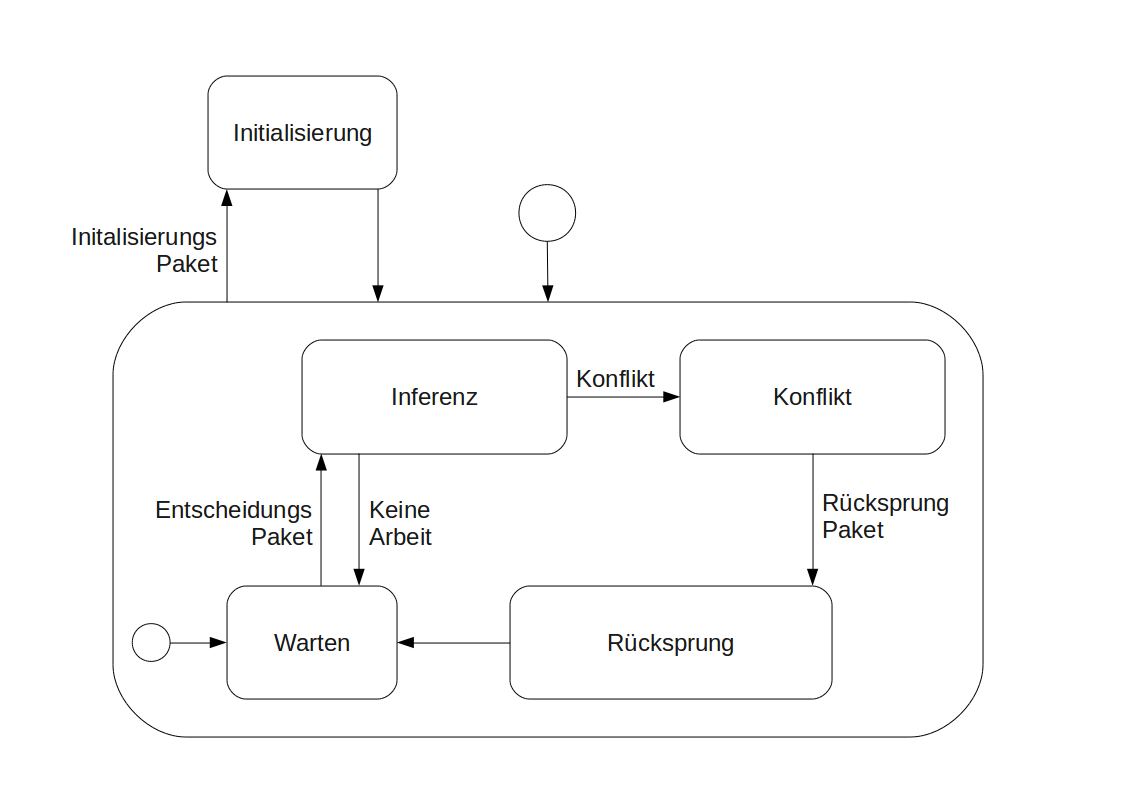
\includegraphics[width=\textwidth]{abb/state-chart.png}
  \caption{FPGA-Zustände}
  \label{modi}
\end{figure}

\subsection{Host-PC}
\label{host_pc}
Der Host-PC führt die softwareseitigen Komponenten (Gruppieren der Formel, Entscheidungsheuristik, 
Konfliktanalyse, Prüfen der Interpretation) des SAT-Solvers durch. 
Dabei kann man hierfür eigentlich jeden DPLL-Solver mit Rücksprung 
ohne Probleme anbinden. In Listing \ref{host_code} ist der benutzte Algorithmus des Host-PCs skizziert.
Es wird eine veränderte Form eines DPLL-Verfahrens genutzt.
Unterstrichen sind dabei die Funktionen, welche direkt mit dem FPGA interagieren.
\newpage
\lstset{
  language=C++, basicstyle=\small \ttfamily, showspaces=false, showtabs=false, tabsize=2 , keywordstyle=\bfseries, 
  showstringspaces=false, framexleftmargin=5mm, frame=single, numbers=left, numberstyle=\tiny, 
  stepnumber=1, numbersep=5pt, texcl=true, captionpos=b, commentstyle=\color{blue}, 
  classoffset=1,morekeywords={init,backtrack,propagate, wait}, keywordstyle=\color{red}\bfseries\underbar,
  classoffset=0}

\begin{lstlisting}[caption=Algorithmus Host-PC, label=host_code]
  
  // Der Algorithmus nimmt eine Formel
  // und gibt eine partielle Interpretation
  // zurück.
  vector<short int> dpll(Formula formula){

    int wait_result;             // Art des empfangenen Pakets
    vector<short int> decisions; // Entscheidungsliterale
    vector<short int> literals;  // Empfangene Literale 
                                 // vom FPGA
    vector<short int> trail;     // Partielle Interpretation
    short int lit = 0;           // Entscheidungsliteral
    short int backtrack_lit = 0; // Rücksprungliteral

    // Die Formel wird gruppiert und
    // an den FPGA geschickt.
    init(group(formula));

    while(1){
      // Warte auf eine Antwort des FPGAs.
      wait_result = wait(literals);

      // Aktualisiere die partielle Interpretation
      // mit den Daten des FPGAs.
      trail.push_back(literals);

      // Auswertung der FPGA-Antwort.
      // Das empfangene Paket ist unbekanntem Typs.
      if(wait_result == -1){
        return 0;
      }
      // Der FPGA hat einen Konflikt festgestellt
      // und muss zurückspringen.
      else if(wait_result == 2){
        backtrack_lit = backtrack(decisions, trail);
        propagate(backtrack_lit);
      }
      // Der FPGA braucht mehr Eingabedaten.
      // Das heißt die Entscheidung für eine
      // Variable muss getroffen werden.
      else if(wait_result == 3){
        lit = decide(interpretation, trail);
        if(lit != -1){
          propagate(lit);
        }
        else{
          // Keine weiteren Literale können entschieden werden.
          break;
        }
        decisions.push_back(lit);
      }
      // Der FPGA hat nur seine Daten geschickt,
      // da eine Sendefifo geleert werden musste.
      else if(wait_result == 4){
      }
    }

    return trail;
  }
\end{lstlisting}
Im Folgenden werden die unterstrichenen Funktionen im Quelltext von Listing \ref{host_code} erläutert:
\begin{itemize}
\item
  \textbf{Init(${\cal G}^{(1)}$)} initialisiert den FPGA, indem eine
  gruppierte Formel Literal für Literal über Ethernet an den FPGA gesendet
  wird. Das Ethernetpaket wird als Initialisierungspaket 
  markiert. Sollte eine neue Gruppe bzw. eine neue Klausel beginnen,
  werden diese Informationen durch bestimmte Steuerkodes im
  Ethernetpaket mitgesendet. Der Aufbau eines solchen
  Initialisierungspakets wird im Unterkapitel zur
  Ethernetschnittstelle beschrieben. Da der Entwurf für 9-SAT
  ausgelegt wurde, werden immer 9 Literale pro Klausel gesendet. 
  Sollte eine Klausel weniger als 9 Literale enthalten, wird 
  diese einfach mit Nullen aufgefüllt. Dies macht die Verarbeitung
  der Daten auf dem FPGA später einfacher, da man von einer 
  festen Klausellänge ausgehen kann.
\item
  \textbf{Propagate($l$)} sendet ein Literal $l$ über Ethernet an
 den FPGA. Das Paket wird als spezielles Entscheidungspaket
 markiert. Das Literal wurde normalerweise vorher durch
 eine Entscheidungsheuristik  bestimmt und war kein
 Element der partiellen Interpretation. Es wäre auch
 möglich, gleich mehrere Literale an den FPGA zu senden, 
 um weiteren Kommunikationsbedarf
 zu vermeiden. Das wäre der Fall,
  wenn nach vollständigem Propagieren weitere Literale angefordert
 werden. Jedoch würde dies
  eine kompliziertere Verwaltungslogik nach sich ziehen.
 So wurde sich bei diesem Entwurf dafür
  entschieden, nur ein Entscheidungsliteral senden und
 verarbeiten zu können.
\item
  \textbf{Backtrack(${l_1, …, l_n}$)} sendet eine Menge von Literalen über Ethernet an den FPGA
  und gibt das negierte letzte Entscheidungsliteral zurück. 
  Das Ethernetpaket wird als Rücksprungpaket markiert. Bei genutztem DPLL Algorithmus entsprechen
  die Literale der partiellen Interpretation bis zum letzten Entscheidungsliteral.\\
  Man könnte hier auch die Möglichkeit eines nonchronological Backtrackings (Backjumping) in 
  Betracht ziehen, wie es bei CDCL-Algorithmen angewandt wird. Dann müssten gelernte Klauseln
  in einer extra Datenstruktur auf dem Host-PC gehalten und separat propagiert werden.
  Außerdem müssten Unit-Literale der gelernten Klauseln dem FPGA mitgeteilt werden, was wieder mehr
  Kommunikationsbedarf bedeuten würde. 
  Die Rücksprungliterale werden auf dem FPGA ähnlich behandelt wie normale Literale, nur
  dass diese keinen Inferenzmechanismus auslösen und aus der partiellen Interpretation
  entfernt werden.

\item
  \textbf{Wait()} wartet auf eine Antwort des FPGAs. Ist das Antwortpaket mit dem 
  Steuerkode 0x02 markiert, dann handelt es sich um ein Konfliktpaket. 
  Alle Literal (jeweils 2\,Byte) die dem Steuerkode folgen sind Teile der partiellen 
  Interpretation und sollten zur partiellen Interpretation des Host-PCs 
  hinzugefügt werden, um diese zu aktualisieren. Das letzte Literal entspricht dabei dem Konflikt-Literal. 
  Ist das Antwortpaket mit 0x03 markiert, dann wartet der FPGA auf mehr Eingabedaten.
  Diese Eingabedaten sind Entscheidungsliterale und werden vom FPGA propagiert.
  Ist das Antwortpaket mit 0x04 markiert, dann wird eine Menge von Literalen gesendet, 
  welche der partiellen Interpretation hinzugefügt werden sollen. Dies geschieht 
  weil ein Sendefifo im FPGA geleert werden muss.
\end{itemize}
In Zeile 16 von Listing \ref{host_code} wird die Gruppierung der Formel F durchgeführt und
das Ergebnis an den FPGA gesendet. Je nach Größe des FPGAs und dem vorhandenen Block-RAM können verschieden viele Gruppen
erzeugt werden. Dabei gilt je mehr Gruppen verfügbar sind, desto größere Probleme kann man lösen.
Es gilt für $group: F \rightarrow {\cal G}^{(1)},\ |{\cal G}^{(1)}| = n$. Wobei die
Anzahl von möglichen Gruppen $n$ von FPGA-Parametern abhängt.\\

\subsection{Ethernet-Schnittstelle}
\label{ethernet}
Es gibt viele Möglichkeiten, um eine Kommunikation zwischen Host-PC
und FPGA zu realisieren. Dabei unterscheiden sie sich zum einen 
in ihrer Bandbreite und Latenz und zum anderen
im Aufwand ihrer Implementierung in Hardware. Sicher wäre eine
Verbindung über PCIe, HT etc. dem einer Ethernetschnittstelle vorzuziehen,
wenn es das Ziel ist, möglichst niedrige Kommunikationslatenzen zu erreichen.
Jedoch lassen sich diese Schnittstellen nur mit viel Aufwand implementieren,
so dass sich für den Prototyp für
Ethernet als Schnittstelle für den Entwurf entschieden wurde. 
Man kann das System auch sehr einfach durch weitere FPGA-Boards erweitern,
da diese nur an das Ethernetnetzwerk angeschlossen werden müssen.\\
Der Host-PC wird mithilfe einer Ethernet-Schnittstelle an den FPGA angebunden. 
Dabei wird ein bereits auf dem FPGA-Board vorhandener Ethernet-MAC-Schaltkreis genutzt. 
Die Kommunikation mit dem Ethernet-MAC erfolgt mittels Local-Link-Interface \cite{xilinxlocallink:2005}. 
Die übermittelten Pakete sind reine Ethernet-Pakete ohne weitere Schichten darüber 
wie Vermittlungs- bzw. Transportschicht. Ein Ethernet-Paket besteht aus einer Folge von 
minimal 64 bis maximal 1522\,Bytes. 
\begin{figure}[h]
  \centering
  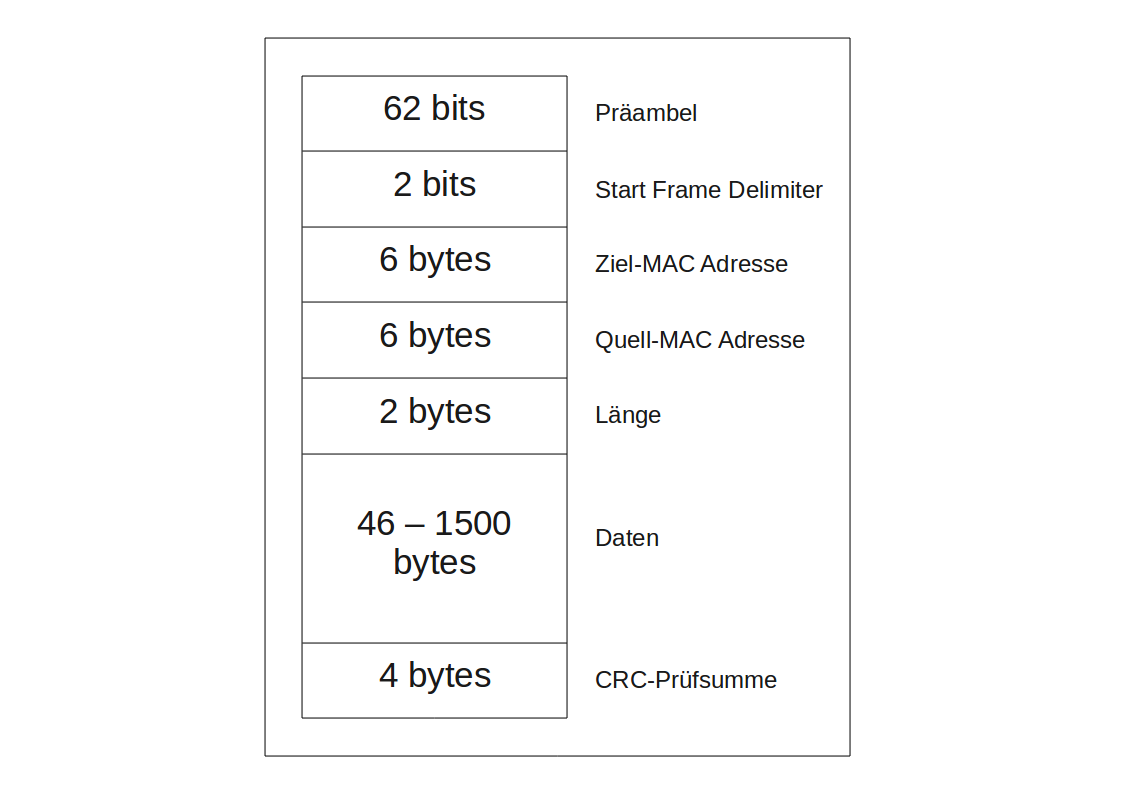
\includegraphics[width=0.75\textwidth]{abb/ethernet.png}
  \caption{Aufbau eines Ethernet-Pakets}
  \label{ether}
\end{figure}
Abbildung \ref{ether} zeigt den Aufbau eines Ethernet-Pakets,
wobei nur Ziel-MAC-Adresse, Quell-MAC-Adresse, Länge und die Daten vom Local-Link-Interface 
empfangen bzw. gesendet werden. Die restlichen Teile des Pakets werden vom 
Ethernet-MAC abgeschnitten bzw. hinzugefügt. Wie bereits im Host-PC-Kapitel erwähnt,  
werden Pakete mit speziellen Steuerkodes markiert um dem jeweiligen Empfänger 
(Host siehe Tabelle \ref{steuerkode2}, FPGA siehe Tabelle \ref{steuerkode1})
mitzuteilen, um welche Art von Paket es sich handelt. Der Steuerkode 
ist immer das erste Byte im Datenbereich des Pakets. Bytes werden in
der Byte-Reihenfolge Big Endian übertragen.
\begin{table}[h]
  \centering
  \begin{tabular}{|l|l|l|}
    \hline
    \textsc{Steuerkode} & \textsc{Bedeutung} & \textsc{Aufbau des Datenteils}\\
    \hline
    \hline
    $ 0x01 $ & Initialisierungspaket & 
    $\langle 0x01 \rangle,((\langle 0x0101 \rangle|\langle 0x0201 \rangle),l_1,l_2, ... , l_9)^+, $\\
    & & $\langle 0x0101 \rangle, (\langle 0x0000 \rangle)^9$\\
    $ 0x02 $ & Entscheidungspaket    & $\langle 0x02 \rangle,l$\\
    $ 0x03 $& Rücksprungpaket     & $\langle 0x03 \rangle ,l_1, ..., ln$\\
    \hline
  \end{tabular}
  \caption{Daten der Pakete vom Host-PC zum FPGA}
  \label{steuerkode1}
\end{table}
Der Aufbau des Initialisierungspakets ist etwas aufwändiger. Jede Klausel wird
Literal für Literal übertragen, jedoch wird vorher noch festgelegt, ob sich die nächste
Klausel in einer neuen Gruppe befindet (durch $0x0201$) oder ob die nächste Klausel in
der gleichen Gruppe ist wie die Klausel davor (durch $0x0101$). Deshalb
muss man darauf achten, die Gruppen in der richtigen Reihenfolge
zu übertragen. Ein Initialisierungspaket wird immer mit einer leeren Klausel
abgeschlossen.
\begin{table}[h]
  \begin{tabular}{|l|l|l|}
    \hline
    \textsc{Steuerkode} & \textsc{Bedeutung} & \textsc{Aufbau des Datenteils}\\
    \hline
    \hline
    $0x02$ & Konfliktpaket        & $\langle 0x02 \rangle (l)^*$\\
    $0x03$ & Eingabepaket         & $\langle 0x03 \rangle (l)^*$\\
    $0x04$ & Aktualisierungspaket & $\langle 0x04 \rangle (l)^*$\\
    \hline
  \end{tabular}
  \caption{Daten der Pakete vom FPGA zum Host-PC}
  \label{steuerkode2}
\end{table}
Die Pakete, welche der FPGA an den Host-PC sendet, ähneln sich im Aufbau sehr,
da mit jedem Paket auch Informationen über propagierte Literale an den 
Host-PC mitgesendet werden können. Die propagierten Literale sind Unit-Literale,
welche während des Inferenzprozessen auf dem FPGA entstanden sind. Die
Literale werden in einem Fifo zwischengespeichert und bei der nächsten 
Gelegenheit in einem Paket vom FPGA zum Host-PC mitgesendet.\\

\subsection{Literal-Arbiter}
\label{arbiter}
Arbiter kommt von \textit{to arbitrate} und heißt \textit{über etwas entscheiden}.
Das beschreibt die Funktion des Literal-Arbiters ganz gut, denn dieses
Modul entscheidet darüber, welches Literal als nächstes propagiert werden soll.
In Abbildung \ref{literal_arbiter} ist der Aufbau des Moduls grob skizziert. 
Signale von links entsprechen dabei Ausgangssignalen
des Ethernet-MAC-Moduls. Signale von rechts sind dementsprechend
Eingangs- bzw. Ausgangssignale der Propagation-Engines.\\
\begin{figure}[h]
  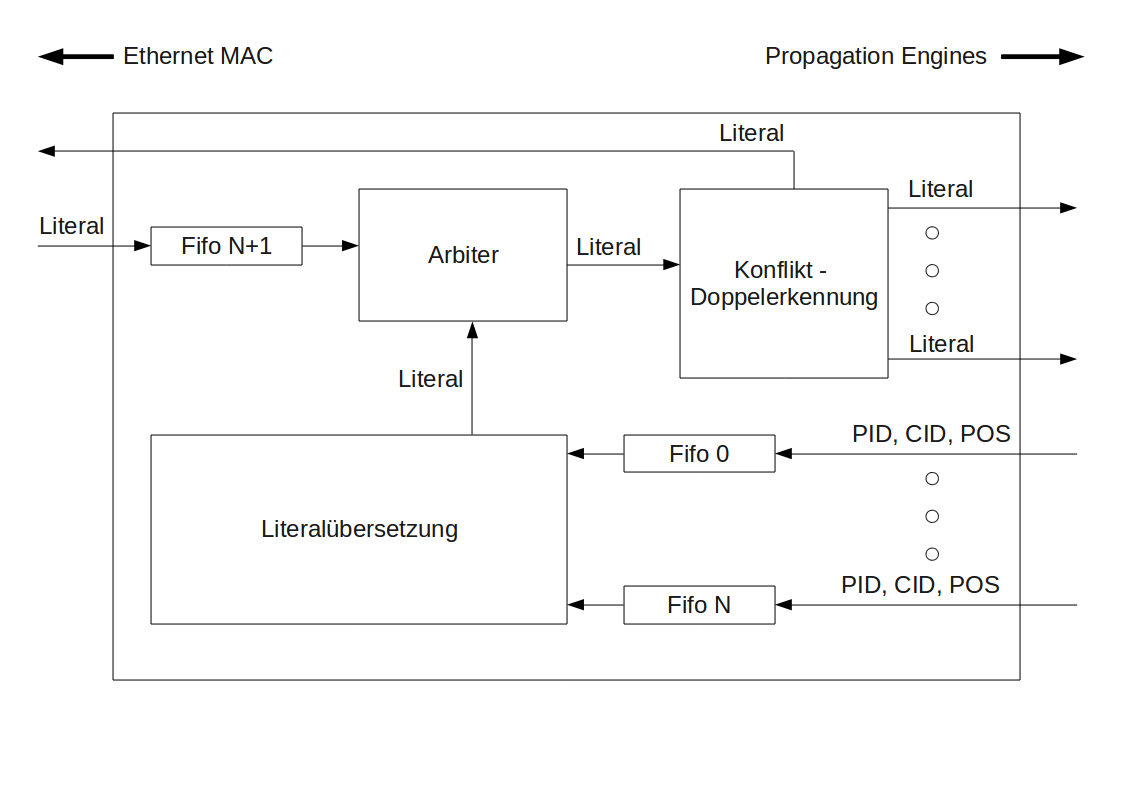
\includegraphics[width=\textwidth]{abb/literal_arbiter.png}
  \caption{Literal-Arbiter}
  \label{literal_arbiter}
\end{figure}Erläuterungen zu Abbildung \ref{literal_arbiter}:
\begin{itemize}
\item
  \textbf{FIFO N+1}\newline
  Dieser Fifo nimmt Entscheidungs- bzw. Rücksprungliterale vom Ethernet-MAC
  entgegen und speichert diese, bis sie weiter verarbeitet werden. Jedes
  Literal führt dabei die Information mit, ob es Entscheidungs- oder
  Rücksprungliteral ist.
\item
  \textbf{FIFO 0 bis N}\newline
  Diese Fifos speichern das Ausgangstupel(PID, CID, POS) von Signalen
  der jeweiligen Propagations- Engines 0 bis N. PID entspricht
  der Propagation-Engine-Identifikationsnummer und
  ist gleich dem Gruppenindex der zugehörigen Gruppe.\\
  CID entspricht der Klausel-Identifikationsnummer und ist innerhalb einer
  Propagation-Engine einmalig. POS entspricht der Position eines Literals innerhalb
  der Klausel, welche mit CID gekennzeichnet ist.
\item
  \textbf{Literal-Übersetzung}\newline
  Dem Tupel (PID, CID, POS) der Fifos 0 bis N werden 
  Literale zugeordnet, um mit diesen wieder Inferenz
  durchführen zu können. Welches Literal welchem Tupel
  zugeordnet wird entscheidet sich bei der Initialisierung
  des FPGAs. Sei die Formel
  $F_{group} = \langle[1,2],[2,3],[3,4],[4,5]\rangle$
  aus dem Gruppen-Einführungskapitel gegeben, dann wurde bereits festgestellt, dass man
  diese Formel in 2 Klauselmengen gruppieren kann. $G_1 = \{[1,2].[3,4]\}$, $G_2 = \{[2,3].[4,5]\}$.
  Zum Beispiel wird dem Literal $l = 2$ der ersten Klausel in $G_2$ das Tupel (2, 1, 1) zugeordnet.
  Die Zuordnungen werden im Block-RAM des FPGAs gespeichert. Bei
  32 Propagation Engines (5\,Bit), 128 Klauseln pro Propagation-Engine (7\,Bit) und
  9 Literalen pro Klausel (4\,Bit) ergibt sich eine 16\,Bit breite Adresse.
  Mit 9\,Bit pro Literal ergibt sich ein Gesamtspeicherbedarf von ca. 590\,kbit 
  ($2^{16}$ x $9$\,Bit) für die Literalübersetzungstabelle.

\item
  \textbf{Arbiter}\newline
  Der Arbiter entscheidet, welches Literal als nächstes propagiert werden soll
  und wählt dabei von den Fifos 0 bis N+1 aus. Es wird der Fifo ausgewählt, 
  welcher nicht leer ist und 
  den kleinsten Index hat. Somit werden Entscheidungsliterale immer
  zuletzt ausgewählt.

\item
  \textbf{Konflikt / Doppelerkennung}\newline
  Der Wahrheitswert jeder Variablen wird in einer partiellen Interpretation gespeichert. 
  Sollte ein Literal bereits interpretiert sein, dann gibt es zwei Möglichkeiten. Stimmt
  der Wahrheitswert des Literals mit dem der partiellen Interpretation überein, dann 
  muss das Literal nicht weiter bearbeitet werden, da es bereits propagiert wurde. 
  Sind die Wahrheitswerte gegensätzlich, dann wurde ein Konflikt gefunden, 
  welcher aufgelöst werden muss. Ein Konflikt wird dem Ethernet-MAC
  mitgeteilt, welcher wiederum den Host-PC informiert.
  Alle Literale, welche noch nicht in der partiellen Interpretation 
  des Host-PCs enthalten sind,
  werden an den Ethernet-MAC übermittelt. Dies ist notwendig, um den 
  Host-PC über den aktuellen Suchprozess zu informieren.
\end{itemize}

\subsubsection{Verhalten des Literal-Arbiters in \\ verschiedenen Zuständen}
Im Literal Arbiter wird prinzipiell zwischen fünf Zuständen unterschieden:
\begin{itemize}
\item
  \textbf{Initialisierungszustand}\\
  Im Initialisierungszustand wird keinerlei Inferenz durchgeführt, sondern nur Speicher initialisiert,
  welcher später von den Algorithmen gebraucht wird. Zum einen muss die Literal-Übersetzungstabelle 
  mit den entsprechenden (PID, CID, POS) zu Literalpaaren gefüllt werden, andererseits muss an die
  Propagation-Engine die Information übermittelt werden, welche Klauseln sie beinhalten. Die
  entsprechenden Signale werden über dedizierte Leitungen direkt in den Block-RAM
  der entsprechenden Module geschrieben.
\item
  \textbf{Inferenzzustand}\\
  Der Inferenzzustand ist der angenommene Normalfall, da es das Ziel
  des Systems ist, Inferenz durchzuführen. Literale werden vom Arbiter ausgewählt,
  von der Konflikt / Doppelerkennung getestet und dann an die Propagation-Engines übermittelt.
  In den Propagation-Engines werden dann die übermittelten Literale propagiert.
  Sollte ein Unit-Literal gefunden werden, dann wird dieses wieder inferiert.
\item
  \textbf{Rücksprungzustand}\\
  Der Rücksprungzustand verhält sich ähnlich zum Inferenzzustand nur das hier keine Konflikt und
  Doppelerkennung stattfindet, sondern die Wahrheitswerte der ausgewählten Literale werden in 
  der partiellen Interpretation auf undefiniert zurückgesetzt.
\item
  \textbf{Konfliktzustand}\\
  Sollte es innerhalb des Inferenzprozesses zu einem Konflikt kommen (erkannt durch
  die Konflikterkennung), dann wird die Bearbeitung weiterer Literale sofort eingestellt.
  Außerdem werden die Fifos 0 bis N+1 und die Fifos in den Propagation-Engines zurückgesetzt.
  Dieser ganze Prozess ähnelt einem Systemweiten Reset,  außer dass die Initialisierten
  Daten und die partielle Interpretation erhalten bleiben. Der Host-PC wird außerdem
  über die Konfliktsituation mit einem Konfliktpaket informiert und muss sich
  um die Konfliktbehandlung kümmern.
\item
  \textbf{Wartezustand}
  Wenn in keiner Propagation-Engine mehr ein Inferenzprozess stattfindet
  und der Literal-Arbiter keine Aufgabe hat, wechselt er in den Wartezustand.
  In diesem Zustand wartet er auf ein Entscheidungspaket vom Host-PC.
  Damit das der Host-PC weiß, wird er mit einem Eingabepaket informiert.
  
\end{itemize}

\subsection{Propagation-Engine}
\label{propagation_engine}
Das Propagation-Engine-Modul ist das eigentliche Herzstück des Entwurfs und führt 
die Inferenz von Literalen durch. Jeder Propagation Engine wird eine Gruppe zugewiesen.
Das heißt in einer Propagation Engine ist eine Variable maximal einmal
in einer Klausel vorhanden. In Abbildung \ref{pe} ist der Aufbau der Propagation Engine 
skizziert. Es werden zwei Hauptmodule unterschieden: das Literal-Lookup-Modul und das
Status-Tabellen-Modul.
\begin{figure}[h]
  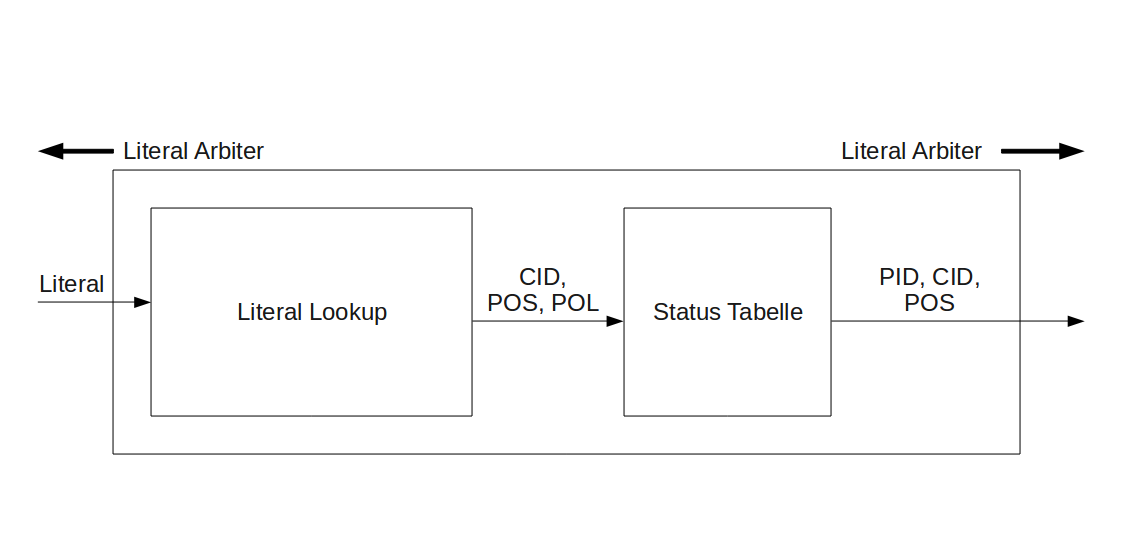
\includegraphics[width=\textwidth]{abb/propagation_engine.png}
  \caption{Propagation-Engine}
  \label{pe}
\end{figure}

\subsubsection{Literal-Lookup}
Das Literal-Lookup-Modul benutzt einen 18\,kbit Block-RAM. 
Damit ist es möglich, einen 10\,Bit Adressraum zu je 18\,Bit
Daten zu erzeugen. Eine Variable entspricht der Adresse des 
Block-RAMs und die Daten an dieser Adresse entsprechen der Klausel,
der Position und der Polarität des entsprechenden Literals (auch Wertetupel
der Variable genannt). Aufgabe des Literal-Lookup-Moduls
ist es, dieses Wertetupel an die Statustabelle weiterzugeben, 
falls es vorhanden sein sollte. Nicht vorhandene Wertetupel
sind im Speicher ausgenullt.
\begin{figure}[h]
  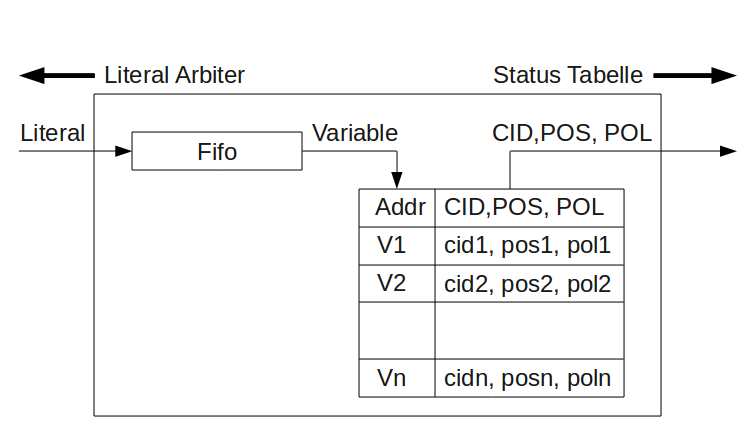
\includegraphics[width=0.75\textwidth]{abb/literal_lookup.png}
  \caption{Literal-Lookup}
  \label{literal_lookup}
\end{figure}
Somit ist die Anzahl der möglichen Variablen auf eine Obergrenze
von $2^{10}-1\ =\ 1023$ festgelegt (wobei die Literalübersetzung
die Variablenanzahl bereits auf 256 beschränkt). Literale werden in einem
Fifo gepuffert, so dass die Propagation-Engines unabhängig voneinander
arbeiten können. In Abbildung \ref{literal_lookup} ist das Literal-Lookup-Modul skizziert.


\subsubsection{Status-Tabelle}
Das Status-Tabellen-Modul benutzt ebenfalls einen 18\,kbit Block-RAM,
jedoch in einer Konfiguration mit einem 11\,Bit Adressraum zu je
9\,Bit Daten. Die Adresse des Block-RAMs entspricht der CID, welche
nur lokal für eine Propagation Engine gilt. Somit gibt es auch
eine Obergrenze von $2^{11} = 2048$ Klauseln pro Propagation Engine
(beschränkt auf 128 wegen Literalübersetzung).
Ein 9 Bit Datenwort entspricht der Interpretation
einer Klausel mit maximal 9 Literalen und wird hier Status genannt. Eine '0' an der Stelle m 
im Status bedeutet, dass das Literal an Position m unter der aktuellen
partiellen Interpretation den Wahrheitswert falsch zugewiesen bekommen hat.
Eine '1' an der Stelle m im Status bedeutet, das der Wahrheitswert des
Literals entweder wahr oder undefiniert ist. Dies wird nicht
unterschieden, da es keinerlei Information über mögliche Inferenz
liefert. Sollte eine Klausel weniger als 9 Literale enthalten, 
dann werden die restlichen Bits bereits beim initialisieren
vorgenullt. Wirklich existierende Literale werden im Status
Initial mit '1' belegt. In Abbildung \ref{status_tabelle}
ist das Status-Tabellen-Modul abgebildet.
\begin{figure}[h]
  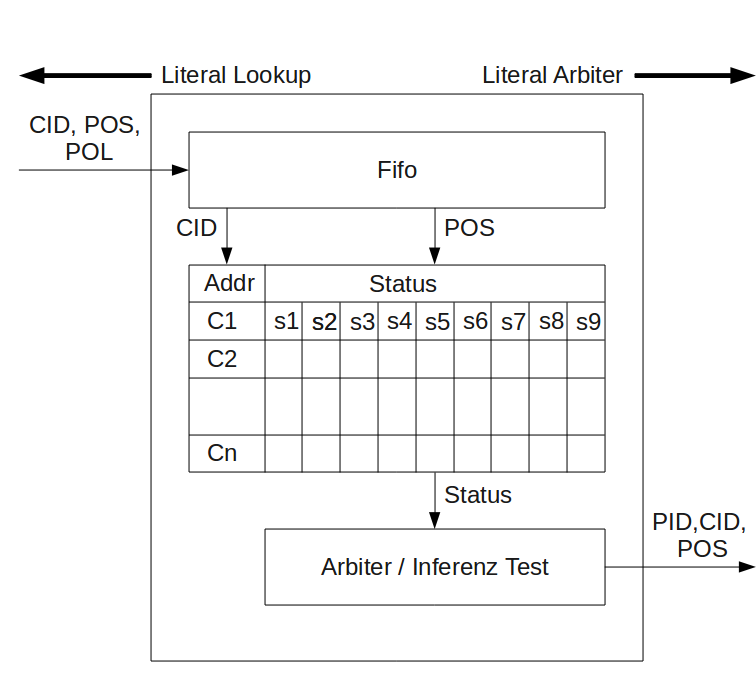
\includegraphics[width=0.75\textwidth]{abb/status_tabelle.png}
  \caption{Status-Tabelle}
  \label{status_tabelle}
\end{figure}

\subsubsection{Inferenz von Literalen}
Um nun herauszufinden, ob eine Klausel durch Propagieren 
eines Literals Unit wird, muss zuerst festgestellt werden, 
in welcher Klausel und an welcher Position sich das Literal
befindet (dies erledigt der Literal Lookup). 
Mit dieser Information kann der Status der Klausel aus dem 
Block-RAM geladen werden (da die Klausel-ID der Block-RAM Adresse
in der Status-Tabelle entspricht). An der Position des
Literals wird eine '0' im Status eingefügt, falls diese
noch nicht vorhanden ist, und es wird geprüft ob, der nun
entstandene Status nur noch eine '1' enthält. Diese Prüfung geschieht mittels
eines Arbiter-Moduls. Das Arbiter-Modul gibt die Position der ersten '1'
im Status als One-Hot-Code zurück. Wenn man nun den invertierten One-Hot-Code
mit dem Status verundet und eine Bitfolge von Nullen herauskommt,
dann wurde ein Unit Literal gefunden.\\
Sei nun wieder folgende Formel $F_{bsp}$ gegeben.
Dann kann diese Formel in 4 Klauselmengen gruppiert werden.
\begin{center}
$F_{bsp} = \langle [1,3],[-2, 5, -6], [-1,-4,6], [-1,-2,-4,5], [-1,2]\rangle$\\
$group(F_{bsp}) = \{\{[1,3],[-2,5,6]\},\{[-1,-4,6]\},\{[-1,-2,-4,5]\},\{[-1,2]\}\}$
\end{center}
Beispielhaft soll nun das Propagieren von zwei Literalen $l_1 = 2$, $l_2 = -5$ 
anhand der Propagation-Engine von Gruppe 1 
$(G_1 = \{[1,3],[-2,5,6]\})$ gezeigt werden. Es befinden sich $l_1$ und $l_2$ 
im Fifo des Literal-Lookup-Moduls und müssen propagiert werden.
Die Lookup-Tabelle von $G_1$ ist in Tabelle \ref{bsp_literal_lookup2} dargestellt.
%% \begin{table}[h]
%%   \centering
%%   \begin{tabular}{|c|c|c|c|}
%%     \hline
%%     \textsc{Variable} & \textsc{CID} & \textsc{POS} & \textsc{POL}\\
%%     \hline
%%     \hline
%%     1 & 1 & 1 & + \\
%%     \hline
%%     2 & 2 & 1 & - \\
%%     \hline
%%     3 & 1 & 2 & + \\
%%     \hline
%%     4 & - & - & - \\
%%     \hline
%%     5 & 2 & 2 & + \\
%%     \hline
%%     6 & 2 & 3 & + \\
%%     \hline
%%   \end{tabular}
%%   \caption{Literal-Lookup-Tabelle von Gruppe 1}
%%   \label{bsp_literal_lookup}
%% \end{table}
Die Wertetupel der Literale werden aus dem Speicher geladen
und an die Status Tabelle weiter geschickt. Die entsprechenden
Zeilen von $l_1$ und $l_2$ sind in Tabelle \ref{bsp_literal_lookup2}
durch Pfeile markiert.
\begin{table}[h]
  \centering
  \begin{tabular}{|c|l|l|l|}
    \hline
    \textsc{Variable} & \textsc{CID} & \textsc{POS} & \textsc{POL}\\
    \hline
    \hline
     1 & 1 & 1 & + \\
    \hline
    \textbf{$\rightarrow$ 2} & 2 & 1 & - \\
    \hline
    3 & 1 & 2 & + \\
    \hline
    4 & - & - & - \\
    \hline
    \textbf{$\rightarrow$ 5} & 2 & 2 & + \\
    \hline
    6 & 2 & 3 & + \\
    \hline
  \end{tabular}
  \caption{Ausgewählte Zeilen von $l_1$ und $l_2$}
  \label{bsp_literal_lookup2}
\end{table}
%\begin{center}
%  $l_1 \rightarrow (1, 1, +)$\\
%  $l_2 \rightarrow (2, 2, +)$
%\end{center}
Die initiale Status-Tabelle von Gruppe 1 ist in Tabelle \ref{bsp_literal_lookup3}
dargestellt. Der Status der ersten Klausel hat an Position eins und zwei eine '1'
- an den restlichen Position eine '0', da beide Literale der Klausel noch
undefiniert sind. Analog dazu hat auch die zweite Klausel an erster bis dritter
Position eine '1' im Status.
\begin{table}[h]
  \centering
  \begin{tabular}{|c|l|l|l|l|l|l|l|l|l|}
    \hline
    \textsc{CID} & \textsc{1} & \textsc{2} & \textsc{3}& \textsc{4}& \textsc{5}& \textsc{6}& \textsc{7}& \textsc{8}& \textsc{9}\\
    \hline
    \hline
    1 & 1& 1& 0& 0& 0& 0& 0& 0& 0 \\
    \hline
    2 & 1& 1& 1& 0& 0& 0& 0& 0& 0 \\
    \hline
  \end{tabular}
  \caption{Status-Tabelle von Gruppe 1}
  \label{bsp_literal_lookup3}
\end{table}
Die Wertetupel von $l_1$ und $l_2$ werden nun auf die Statustabelle
angewandt (siehe Tabelle \ref{bsp_literal_lookup4}).
Das heißt in Zeile 2 der Statustabelle werden Positionen eins und zwei genullt.
Das Ergebnis ist der Status (001000000). Der Arbiter gibt nun die Position
der ersten '1' als One-Hot-Code zurück (001000000). Verundet man den negierten 
One-Hot-Code mit dem Status erhält man (000000000), was bedeutet, dass
an Position 3 dieser Klausel ein Unit-Literal gefunden wurde.
\begin{table}[h]
  \centering
  \begin{tabular}{|c|l|l|l|l|l|l|l|l|l|}
    \hline
    \textsc{CID} & \textsc{1} & \textsc{2} & \textsc{3}& \textsc{4}& \textsc{5}& \textsc{6}& \textsc{7}& \textsc{8}& \textsc{9}\\
    \hline
    \hline
    1 & 1& 1& 0& 0& 0& 0& 0& 0& 0 \\
    \hline
    2 & \textbf{0}& \textbf{0}& 1& 0& 0& 0& 0& 0& 0 \\
    \hline
  \end{tabular}
  \caption{Status-Tabelle von Gruppe 1 nach propagieren von $l_1$ und $l_2$}
  \label{bsp_literal_lookup4}
\end{table}
Es ist noch nicht bekannt, um welches Literal es sich genau
handelt, man weiß nur sein Identifikationstupel (PID,CID,POS).
Für eine weitere Inferenz des gefundenen Unit-Literals
wird das Tupel (1,2,3) an den Literal-Arbiter weitergeleitet
und dort zurückübersetzt. Man weiß das sich in
der ersten Gruppe in der zweiten Klausel an dritter Position
ein Unit Literal befindet.
